\subsection{Diskrete Signale}

Wir sind nun endlich im Digitalen angekommen. 
Wir wollen uns als erstes verschiedene M"oglichkeiten der Klassifikation von diskreten Signalen $x[\cdot] : \Z \rightarrow \C$ ansehen.
Dabei folgend wir weitestgehend~\cite[Kap.~2.1]{proakis2013}.
In \cref{sec:spec_sig} haben wir bereits den Einheitssto"s $\delta[\cdot]$ und die Heavy-Side-Funktion $u[\cdot]$ kennengelernt.

\begin{itemize}
    \item Eine linear ansteigende Version $u_r[\cdot]$ von $u[\cdot]$ is gegeben durch
    \[
        u_r[n] = n \cdot u[n] = \begin{cases}
            n, \Text{f"ur} n \geqslant 0 \\
            0, \Text{sonst}.
        \end{cases}
    \]
    In Python ist die Funktion auch sehr einfach zu implementieren:
\begin{minted}{python3}
def u_r(n: int) -> int:
    return n if n>0 else 0
\end{minted}
Will man die Funktion effizienter mittels Numpy~\cite{numpy} implementieren, dann liest sie sich
\begin{minted}{python3}
import numpy as np
def u_r_np(n: np.ndarray[int]) -> np.ndarray[int]:
    u_r = n.copy()
    u_r[n <= 0] = 0
    return u_r
\end{minted}
\item F"ur eine komplexe Zahl $a = r \exp(\jmath \theta) \in \C$ erh"alt man das zugeh"orige exponentielle Signal als
\[
    x[n] 
        = a ^ n 
        = r^n \exp(\jmath \theta n) 
        = r^n \cos(\theta n) + \jmath r^n \sin(\theta n).
\]
Damit gilt $x[0] = 1$ unabh"angig von $a$.
Beispielsweise erhalten wir das Signal $x_k$ aus \eqref{eq:disc_harms_comp} indem wir $r=1$ und $\theta = 2 \pi k f_0$ setzen.
Eine Implementierung von $x[n]$ is in \Cref{py:complex_exp} gegeben.
Es ist sicher interessant f"ur verschiedene Werte von $a$ und $\bm n$ die Ausgabe zu betrachten.

Beispielsweise kann man sehen, dass f"ur $a \in \R$ gelten muss, dass $\lim_{n \rightarrow \infty} x[n] = 0$, falls $a < 0$, aber $\lim_{n \rightarrow -\infty} x[n] = \infty$.
Weiterhin gilt f"ur $a \in \C$ und $\Abs{a} = 1$, dass dann auch $\Abs{x[n]} = 1$ f"ur alle $n$.
\end{itemize}
%
\begin{listing}
    \noindent
    \begin{minipage}{0.49\textwidth}
        \strut\vspace*{-\baselineskip}\newline
        \inputminted[firstline=4]{python3}{code/complex_exp.py}
    \end{minipage}%
    \begin{minipage}{0.49\textwidth}
        \strut\vspace*{-\baselineskip}\newline
        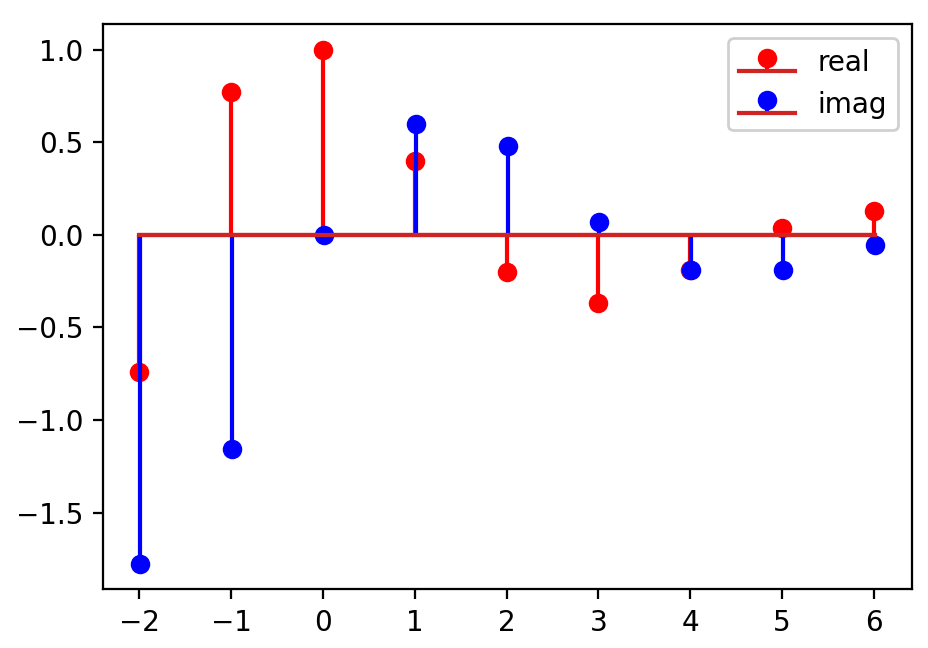
\includegraphics[width=\textwidth]{code/complex_exp.png}
    \end{minipage}
    \codecaption{code/complex_exp.py}{Berechnung und Darstellung eines komplexen exponentiellen Signals}\label{py:complex_exp}
\end{listing}
%
\subsubsection{Energie Diskreter Signale}

Oft ist es interessant zu bemessen, wie viel Energie in einem Signal vorhanden ist.
Hierzu betrachten wir
\begin{equation}\label{eq:disc_sig_energy}
    E(x[\cdot]) 
        = \Sum{n \in \Z}{}{\Abs{x[n]}^2} 
        = \Sum{n \in \Z}{}{x[n]^\ast \cdot x[n]}.
\end{equation}
Wenn gilt $E(x[\cdot]) < \infty$, dann sprechen wir erstaunlicherweise von einem Signal endlicher Energie.

Es ist nun interessant sich eine Menge $\mathcal{E}$ zu definieren, die alle Signale enth"alt, welche endliche Energie besitzen, also 
\[
    \mathcal{E} = \{x : \Z \rightarrow \C \Text{mit} E(x[\cdot]) < \infty\}.
\]
Man kann sich nun "uberlegen, dass
\[
E(\alpha x[\cdot] + \beta y[\cdot]) 
    \leqslant E(\alpha x[\cdot]) + E(\beta y[\cdot])
    = \alpha^2 E(x[\cdot]) + \beta^2 E(y[\cdot]) 
    < \infty 
\]
gelten muss, falls $E(x[\cdot]),E(y[\cdot]) < \infty$. 
Das hei"st, dass Linearkombinationen von Signalen mit endlicher Energie wieder ein Signal mit endlicher Energie ergeben.
Das hei"st, dass die Signale endlicher Energie bilden einen \emph{Unterraum}.
Wir k"onnen noch einen Schritt weiter gehen und wie in \eqref{eq:dtft_inner_prod} die Summe in \eqref{eq:disc_sig_energy} als Skalarprodukt auffassen.

Definieren wir f"ur zwei Signale endlicher Energie die Abbildung $\ScPr{\cdot}{\cdot} : \mathcal{E} \times \mathcal{E} \rightarrow \C$ als
\begin{equation}\label{eq:disc_inner_prod}
    (x[\cdot], y[\cdot]) 
        \mapsto \ScPr{x[\cdot]}{y[\cdot]}
        = \Sum{n \in \Z}{}{x[n]^\ast \cdot y[n]},
\end{equation}
dann kann man sich "uberlegen, dass dies die Bedingungen an ein \emph{Skalarprodukt} erf"ullt.
Beispielsweise kann man sich "uberlegen, dass die unendliche Summe in \eqref{eq:disc_inner_prod} immer endlich ist, falls $x[\cdot], y[\cdot] \in \mathcal{E}$, da
\[
\Abs{\ScPr{x[\cdot]}{y[\cdot]}} \leqslant E(x[\cdot]) \cdot E(y[\cdot]) < \infty
\]
Nun kann man aber auch $E$ durch
\[
E(x[\cdot]) = \ScPr{x[\cdot]}{x[\cdot]}
\] 
ausdr"ucken.

\begin{Bsp}
Betrachten wir $x[n] = a^n \cdot u[n]$ f"ur $a = r \exp{\jmath \theta} \in \C$.
Dann berechnet sich $E(x[\cdot])$ durch
\[
E(x[\cdot]) 
    = \Sum{n \geqslant 0}{}{\Abs{a^n}^2} 
    = \Sum{n \geqslant 0}{}{\left(r^2\right)^n}
\]
Ist nun $r \geqslant 1$, dann $E(x[\cdot]) = \infty$, falls aber $r < 1$, dann ergibt sich aus der geometrischen Reihe, dass
\[
    E(x[\cdot]) = \frac{1}{1 - r^2}
\]
gilt.
Das hei"st auch, dass das Heavy-Side-Signal $u[\cdot]$ keine endliche Energie besitzt.
\end{Bsp}
%
\subsubsection{Periodische Signale}
%
Gilt f\"ur ein Signal $x[\cdot]$, dass $x[n + N] = x[n]$ f"ur ein $N \in \N$ und \emph{alle} $n \in \Z$, so nennt man $x[\cdot]$ periodisch mit Periodenl"ange/Periode $N$, oder kurz $N$-periodisch.
Falls $x[\cdot]$ nun $N$-periodisch ist, dann ist $x[\cdot]$ auch $kN$-periodisch, falls $k \in \N$.
Das hei"st, dass es sinnvoller ist, das \emph{kleinste} $N \in \N$ zu betrachten, sodass $x[\cdot]$ dann $N$-periodisch ist. 
Man nennt $N$ dann Fundamentalperiode.
Falls solch ein $N$ nicht existiert, dann nennt man $x[\cdot]$ aperiodisch, oder nicht-periodisch.
Falls $x[\cdot] \neq 0$, dann gilt f"ur periodische Signale, dass $E(x[\cdot]) = \infty$.
Beispielsweise haben wir bereits in \Cref{sec:sample_harm} gesehen, dass
\[
x[n] = \exp(\jmath 2 \pi f)
\]
periodisch mit Periode $N$ ist, falls $f = k/N$, also eine rationale Zahl ist.
%
\subsubsection{Symmetrie von Signalen}
%
Gilt f"ur ein Signal $x[n] = x[-n]$, dann nennt man es \emph{symmetrisch} bzw.~\emph{gerade}.
Gilt andererseits $x[n] = -x[-n]$, so nennt man es \emph{anti-symmetrisch} bzw.~\emph{ungerade}.

Ist ein beliebiges Signal $x[\cdot]$ gegeben, so kann man
\[
    x_g[n] = \frac 12 \left(x[n] + x[-n]\right)
    \Text{und}
    x_u[n] = \frac 12 \left(x[n] - x[-n]\right)
\]
definieren.
Dann ist $x_g[\cdot]$ gerade und falls $x[\cdot]$ bereits gerade ist, so gilt $x[\cdot] = x_e[\cdot]$.
Genauso ist $x_u[\cdot]$ ungerade und falls $x[\cdot]$ bereits ungerade ist, so gilt $x[\cdot] = x_u[\cdot]$.
Au"serdem gilt
\[
x[n] = x_g[n] + x_u[n].
\]
Wir haben das Signal $x[\cdot]$ also in einen geraden und einen ungeraden Teil zerlegt.
Wie man an \Cref{py:even_odd} gut sehen kann, muss gelten $x_u[0] =0$, $x_u[0] = x[0] - x[0] = 0$.
%
\begin{listing}
    \noindent
    \begin{minipage}{0.49\textwidth}
        \strut\vspace*{-\baselineskip}\newline
        \inputminted[firstline=4]{python3}{code/even_odd.py}
    \end{minipage}%
    \begin{minipage}{0.49\textwidth}
        \strut\vspace*{-\baselineskip}\newline
        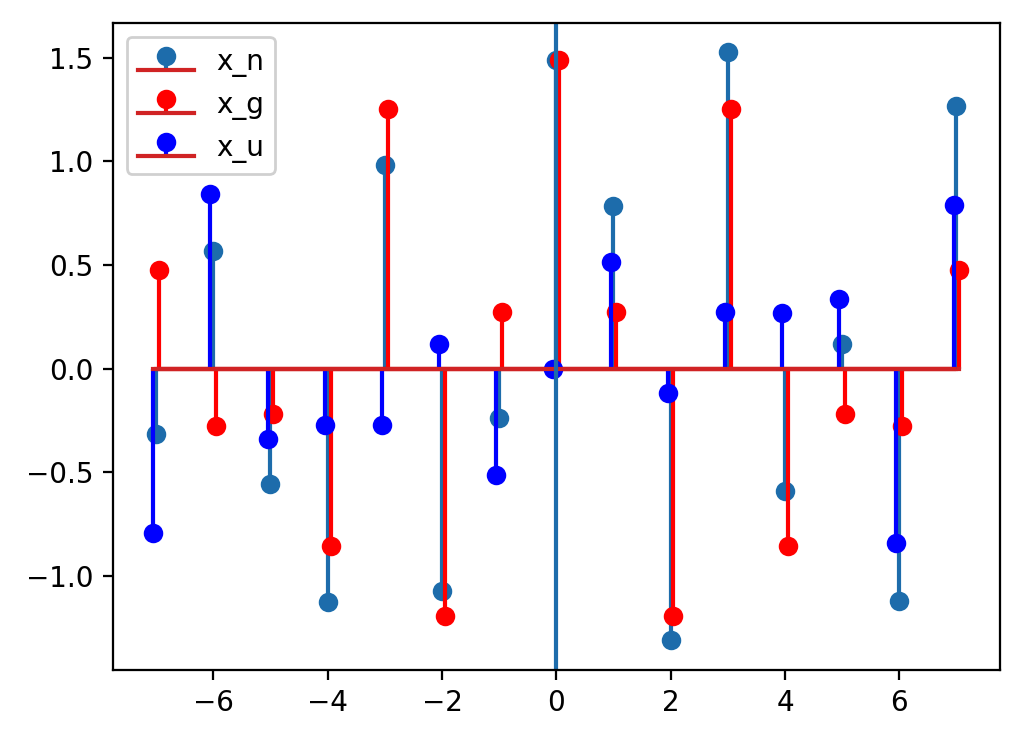
\includegraphics[width=\textwidth]{code/even_odd.png}
    \end{minipage}
    \codecaption{code/even_odd.py}{Zerlegung eines Signals in seinen geraden und ungeraden Anteil.}\label{py:even_odd}
\end{listing}
%
\subsection{Diskrete Systeme}
\begin{itemize}
    \item JEDE manipulation eines signals kann als system aufgefasst werden
    \item system $\mathcal{T}$ ist als abbildung zu verstehen. signal rein, anderes signal raus: $y[n] = (\mathcal{T}x)[n]$ (auf bedeutung von schreibweise eingehen)
    \item beispiele: \cite[ex. 2.2.1]{proakis2013} (a-c vorlesung, rest uebung)
    \item vergangenheit der systeme: akkumulator
    \item blockschaltbilder: adder, multiplikator, scaler, delay, uebung \cite[ex 2.2.3]{proakis2013}(per hand, per modularem code)
    \item statisch vs. dynamisch (gedaechtnislos, mit gedaechtnis)
    \item causal, antikausal, relaxed state
    \item stabilitaet
    \item zeitvariant vs zeitinvariant: definition
\end{itemize}

\subsection{Diskrete \texorpdfstring{\acrshort{lti}}{LTI} Systeme}\label{disc_lti}

\begin{itemize}
    \item wiederholung der eigenschaften: shift-invarianz, linearitaet
    \item reaktion auf signal, das aus bausteinsignalen zusammengesetzt wurde
    \item darstellung als summe von skalierten, geshifteten einheitsstoessen
    \item faltungsformel
    \item algorithmus zur berechnung
    \item exerzieren von beispiel 2.3.2, uebung programmieren (naiv summieren, scipy convolve)
    \item exerzieren von beispiel 2.3.3, uebung programmieren der approximation
    \item assoziativitaet, kommmutativitaet
    \item cascadierung von mehreren systemen
    \item stabilitaet: $h[n]$ muss absolut summierbar sein, gegen $0$ gehen
    \item beispiel 2.3.6. (fuer uebung irgendwas ausdenken)
\end{itemize}

\subsection{Cross- und Autokorrelation}\label{corr}

\begin{itemize}
    \item Definition
    \item eigenschaften
    \item synthetisches beispiel schwingung + noise, akf zeigt periodizitaet
    \item beispiel mit woelfer sunspot numbers
    \item beispiel mit m-sequenzen, niklas einladen, schaltung zeigen
    \item monster uebung: 2.65
\end{itemize}